\documentclass[tikz,border=3pt]{standalone}
\usepackage[utf8]{inputenc}
\usepackage[T1]{fontenc}
\usepackage{lmodern}
\renewcommand{\familydefault}{\sfdefault}
\usepackage{sansmath}\sansmath
\usepackage{chemfig}
\usepackage{pgfplots}\pgfplotsset{compat=1.18,/pgf/number format/use comma,/pgf/number format/1000 sep={.}}
\usetikzlibrary{arrows.meta,calc,positioning,decorations.pathmorphing,patterns}
% paleta del sitio
\definecolor{nar}{HTML}{E8680C}\definecolor{narc}{HTML}{FFB35C}\definecolor{hielo}{HTML}{FFF3E8}
\definecolor{tinta}{HTML}{1D1D1F}\definecolor{gris}{HTML}{6E6E73}\definecolor{lila}{HTML}{7C5CF0}
\definecolor{azul}{HTML}{2F6FD6}\definecolor{menta}{HTML}{17A673}\definecolor{coral}{HTML}{E8342A}
\begin{document}
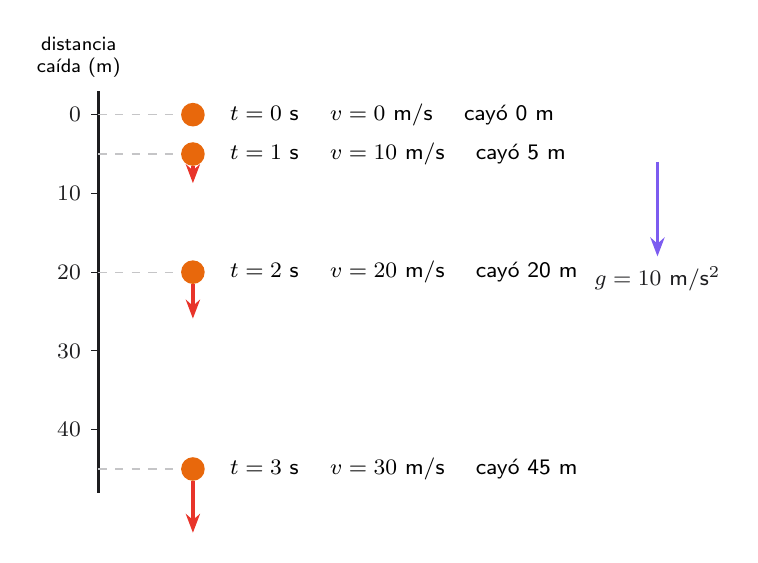
\begin{tikzpicture}[font=\footnotesize,>={Stealth[length=2.4mm]},]
\draw[thick,tinta] (-1.2,0.3) -- (-1.2,-4.8);
\draw[tinta] (-1.2,0.0) -- ++(-0.1,0) node[left] {$0$};
\draw[tinta] (-1.2,-1.0) -- ++(-0.1,0) node[left] {$10$};
\draw[tinta] (-1.2,-2.0) -- ++(-0.1,0) node[left] {$20$};
\draw[tinta] (-1.2,-3.0) -- ++(-0.1,0) node[left] {$30$};
\draw[tinta] (-1.2,-4.0) -- ++(-0.1,0) node[left] {$40$};
\node[above,align=center,font=\scriptsize] at (-1.45,0.35) {distancia\\caída (m)};
\draw[gris!40,dashed] (-1.2,0.0) -- (0,0.0);
\fill[nar] (0,0.0) circle (0.15);
\node[right] at (0.35,0.0) {$t = 0$ s \quad $v = 0$ m/s \quad cayó 0 m};
\draw[gris!40,dashed] (-1.2,-0.5) -- (0,-0.5);
\fill[nar] (0,-0.5) circle (0.15);
\draw[->,very thick,coral] (0,-0.65) -- ++(0,-0.21999999999999997);
\node[right] at (0.35,-0.5) {$t = 1$ s \quad $v = 10$ m/s \quad cayó 5 m};
\draw[gris!40,dashed] (-1.2,-2.0) -- (0,-2.0);
\fill[nar] (0,-2.0) circle (0.15);
\draw[->,very thick,coral] (0,-2.15) -- ++(0,-0.43999999999999995);
\node[right] at (0.35,-2.0) {$t = 2$ s \quad $v = 20$ m/s \quad cayó 20 m};
\draw[gris!40,dashed] (-1.2,-4.5) -- (0,-4.5);
\fill[nar] (0,-4.5) circle (0.15);
\draw[->,very thick,coral] (0,-4.65) -- ++(0,-0.6599999999999999);
\node[right] at (0.35,-4.5) {$t = 3$ s \quad $v = 30$ m/s \quad cayó 45 m};
\draw[->,very thick,lila] (5.9,-0.6) -- (5.9,-1.8) node[below,text=tinta] {$g = 10$ m/s$^2$};
\end{tikzpicture}
\end{document}
